% Author: Till Tantau
% Source: The PGF/TikZ manual
\documentclass[a4paper,11pt]{article}
\usepackage[utf8]{inputenc}
\usepackage{listings}
\usepackage{amsmath}    % need for subequations
\usepackage{graphicx}   % need for figures
\usepackage{verbatim}   % useful for program listings
\usepackage{color}      % use if color is used in text
%\usepackage{subfigure}  % use for side-by-side figures
\usepackage{hyperref}   % use for hypertext links, including those to external documents and URLs
\usepackage{url}
\usepackage{float}
\usepackage{todonotes}
\usepackage{tikz}
\usepackage{enumitem}
\usepackage{hyperref}
\usepackage{pdfpages}
\usepackage{caption}
\usepackage{subcaption}
\usepackage{listings}
\usepackage{color}
\usepackage{amsfonts}
\usepackage{latexsym}
\usepackage[T1]{fontenc} % use for allowing < and > in cleartext
\usepackage{fixltx2e}    % use for textsubscript
\usepackage[linesnumbered,boxed,ruled]{algorithm2e}
% \newcommand{\BigO}[1]{\ensuremath{\operatorname{O}\left(#1\right)}}
\newcommand{\BigO}[1]{\ensuremath{\mathop{}\mathopen{}\mathcal{O}\mathopen{}\left(#1\right)}}
\graphicspath{ {./images/} }
\definecolor{mygreen}{rgb}{0,0.6,0}
\definecolor{mygray}{rgb}{0.5,0.5,0.5}
\definecolor{mymauve}{rgb}{0.58,0,0.82}
\lstset{ %
  backgroundcolor=\color{white},   % choose the background color; you must add \usepackage{color} or \usepackage{xcolor}
  basicstyle=\footnotesize,        % the size of the fonts that are used for the code
  breakatwhitespace=false,         % sets if automatic breaks should only happen at whitespace
  breaklines=true,                 % sets automatic line breaking
  captionpos=b,                    % sets the caption-position to bottom
  commentstyle=\color{mygreen},    % comment style
  deletekeywords={...},            % if you want to delete keywords from the given language
  escapeinside={\%*}{*)},          % if you want to add LaTeX within your code
  extendedchars=true,              % lets you use non-ASCII characters; for 8-bits encodings only, does not work with UTF-8
  %frame=single,                    % adds a frame around the code
  keepspaces=true,                 % keeps spaces in text, useful for keeping indentation of code (possibly needs columns=flexible)
  keywordstyle=\color{blue},       % keyword style
  language=Octave,                 % the language of the code
  morekeywords={*,...},            % if you want to add more keywords to the set
  numbers=left,                    % where to put the line-numbers; possible values are (none, left, right)
  numbersep=5pt,                   % how far the line-numbers are from the code
  numberstyle=\tiny\color{mygray}, % the style that is used for the line-numbers
  rulecolor=\color{black},         % if not set, the frame-color may be changed on line-breaks within not-black text (e.g. comments (green here))
  showspaces=false,                % show spaces everywhere adding particular underscores; it overrides 'showstringspaces'
  showstringspaces=false,          % underline spaces within strings only
  showtabs=false,                  % show tabs within strings adding particular underscores
  stepnumber=2,                    % the step between two line-numbers. If it's 1, each line will be numbered
  stringstyle=\color{mymauve},     % string literal style
  tabsize=2,                       % sets default tabsize to 2 spaces
  %title=\lstname                   % show the filename of files included with \lstinputlisting; also try caption instead of title
}

\bibliographystyle{plain}
\begin{document}

\date{May 18th 2014\\ IT University of Copenhagen}
\title{Assignment 3 - Shading\\SIGB Spring 2014}

\author{Marcus Gregersen\\
\texttt{mabg@itu.dk}
\and Martin Faartoft\\
\texttt{mlfa@itu.dk}
\and Mads Westi\\
\texttt{mwek@itu.dk}}
\clearpage\maketitle
\thispagestyle{empty}
\setcounter{page}{1}
\newpage

% \begin{figure}[H]
% \centering
% \begin{subfigure}{.4\textwidth}
%   \centering
%   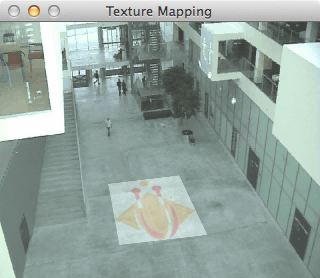
\includegraphics[width=0.8\linewidth]{groundfloor1}
%   \label{fig:floor1}
% \end{subfigure}
% \begin{subfigure}{.4\textwidth}
%   \centering
%   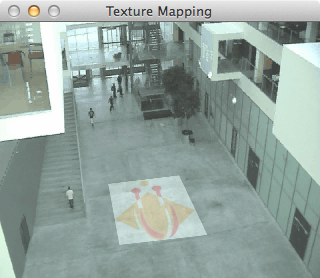
\includegraphics[width=0.8\linewidth]{groundfloor2}
%   \label{fig:floor2}
% \end{subfigure}
% \caption{Linear texture mapping to sequence}
% \label{fig:floor}
% \end{figure}

\section{Introduction}
In this report, we will implement and document a simple shader, able to render a textured cube, and shade it realistically.

\section{Back-Face Culling}
When we render the cube, at most 3 of the faces will be visible to camera, regardless of the positions of cube and camera. Attempting to render all 6 will waste a lot of performance, and furthermore require us to render the faces in the correct order, to get the correct perspective.\todo{eksempelbillede uden culling}

The idea behind back-face culling, is to calculate the dot-product between the camera view vector, and each of the face normals. If the result is negative, the face should be drawn - otherwise it faces away from the camera, and should be discarded.
\[cos(\theta) = V_{view} \cdot \hat{F}\]
Because the cube is convex, back-face culling is sufficient to ensure the scene will be rendered correctly, assuming that the cube is the only object in the scene.

\section{Illumination}
The first step in realistic shading, is to calculate the intensity of the light going towards the camera, from each point on each object in the scene. 

%todo global illumination model (ray-tracing): slow but realistic
%Phong: local illumination model: fast and "good enough" for most uses, but does not correctly model inter-object reflections (mirror facing mirror)
We use the Phong illumination model for this, it calculates the illumnation as:
\[I_{Phong} = I_{ambient} + I_{diffuse} + I_{specular}\]
In the following we will describe how to calculate each component of the Phong illumination model.
\subsection{Ambient Reflection}
Ambient reflection is used when we want all parts of the scene to be illuminated. Without ambient reflection, any point not hit by light from a light source will simply be black.
\[I_{ambient}(x) = I_a \cdot k_a(x)\]
Where $x$ is the point calculating the intensity for $I_a$ is the intensity of the ambient light in the scene, and $k_a(x)$ is the material properties in $x$.

\subsection{Diffuse Shading / Lambertian Reflection}

\subsection{Specular Reflection}

\section{Shading}

\subsection{Flat Shading}
\subsection{Phong Shading}

\section{Conclusion}

\newpage
\section*{Appendix}
\url{https://github.com/MartinFaartoft/sigb}
\subsection*{Assignment\_Cube.py}
\lstinputlisting[language=Python]{../ass2/Assignment_Cube.py}


\end{document}
